\documentclass[10pt]{article}

\usepackage{spheric}
%%%TITLE
\title{Implement of the MPS-FEM coupled method for the FSI simulation of the 3-D dam-break problem}
\date{}

%%AFFILIATIONS

\author[$\relax$]{Youlin Zhang}
\author[$\relax$]{Decheng Wan$^\dagger$}

\affil[$\relax$]{State Key Laboratory of Ocean Engineering, School of Naval Architecture, Ocean and Civil Engineering, Shanghai Jiao Tong University, Collaborative Innovation Center for Advanced Ship and Deep-Sea Exploration, Shanghai 200240, China}

\affil[$\relax$]{\email{\dagger}{dcwan@sjtu.edu.cn}}


%%DOCUMENT
\begin{document}

\maketitle

%\SelectedTopics{}

%%PLEASE PUT YOUR ABSTRACT HERE
\begin{abstract}
The fluid structure interaction (FSI) problems with violent free surface have gained great attentions since they are often encountered in many engineering applications, such as the liquid sloshing in an oil tanker, very large floating structure interacting with waves, flexible structures experiencing dam-break flows, etc. In the past decades, the grid-based methods are much popular in the contributions regarding the simulation of FSI problems. However, it's quite a challenge for such methods to model phenomena that involve complex free surface flows, large deformations of flexible structures. By contrast, the mesh-less methods are free from these difficulties. Therefore, the mesh-less methods, cooperating with the finite element method (FEM), are promising for the FSI problems involving flexible structures and free surface flows.

The current article presents a partitioned approach for the 3-D FSI problems in which the moving particle semi-implicit (MPS) method is coupled with the FEM method. Herein, the MPS method is employed for the simulation of fluid domain while the FEM approach is used for the analysis of structural domain. For the implement of the coupling approach, we proposed a mapping algorithm to transfer quantity values between the particles of flow field and the elements of structural field. In this mapping algorithm, the nonmatching refinement levels of both domains are permitted, which implies that the much larger size of element can be used in the FSI simulation and the computational efficiency can be improved.

With the benefit of the proposed MPS-FEM coupled method, the 3-D FSI problem of dam-break flow impacting onto the flexible wall is numerically investigated. The evolutions of free surface and the impacting loads on the wall are comparative against those regarding rigid tank, as shown in figure \ref{fig:19}. In addition, the deformation and the strength behaviors of the flexible wall are exhibited.

\begin{figure}[!htb]
\begin{minipage}[b]{0.46\linewidth}
\centering
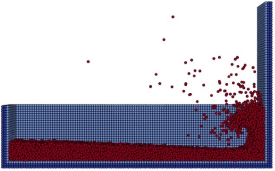
\includegraphics[width=\textwidth]{19-11.png}\\
(a) rigid tank
\end{minipage}
\begin{minipage}[b]{0.05\linewidth}
~
\end{minipage}
\begin{minipage}[b]{0.46\linewidth}
\centering
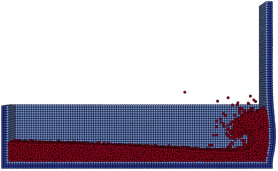
\includegraphics[width=\textwidth]{19-12.png}\\
(b) elastic tank
\end{minipage}
\caption{Comparison of free surface between rigid and elastic tanks}\label{fig:19}
\end{figure}

\end{abstract}


%%THE END OF ABSTRACT

\addbib

\end{document}
